
\chapter{基于技能嵌入的人形机器人分层全身控制}


\section{引言}
在复杂环境中执行任务时，类人机器人往往需要在保证运动稳定性的同时完成多种行为模式的切换，例如移动、操作以及姿态调整等。传统强化学习方法通常针对单一任务或单一运动模式进行训练，这种方式虽然能够在特定任务中取得较好的控制效果，但往往缺乏通用性。当任务场景发生变化或需要执行新的动作组合时，往往需要重新训练控制策略，从而限制了策略在实际应用中的可扩展性与泛化能力。此外，在实际运行过程中，机器人还可能受到外部扰动而发生跌倒，如果缺乏有效的恢复机制，机器人将难以继续执行任务。因此，如何在保证控制稳定性的基础上，实现多种运动技能的灵活组合，并提升系统整体的鲁棒性，是类人机器人全身控制中的重要问题。


在类人机器人全身控制研究中，一个核心问题是如何构建能够稳定执行多种复杂动作的通用动作控制器。早期基于强化学习或模仿学习的方法通常采用单个策略对应单个技能的训练范式，即针对行走、奔跑、跳跃、翻滚或起身等动作分别训练独立控制策略\cite{peng2018deepmimic,heess2017emergence,hwangbo2019learning}。虽然该类方法在单一动作跟踪精度和控制稳定性方面能够取得良好效果，但其显著局限在于：不同动作需要分别设计奖励函数并独立训练策略，导致策略之间缺乏统一表示，难以复用，也难以扩展到包含大量行为模式的复杂任务场景。


随着大规模动作捕捉数据集以及并行物理仿真技术的发展，研究者开始探索能够统一跟踪多种动作的通用控制策略，即从\textbf{单策略学习单一技能}逐步发展为\textbf{单策略学习多种技能}的控制范式。围绕这一目标，现有研究大致形成了三类主要技术路线：多动作强化学习方法、专家策略蒸馏方法以及基于生成模型的策略学习方法。

第一类方法是基于多动作强化学习的统一训练方法。该类方法通常利用包含多种动作片段的参考动作数据集，通过单一策略同时跟踪不同动作，从而获得具有通用性的动作跟踪控制器。例如，GMT\cite{chen2025gmt}、OmniH2O\cite{he2024omnih2o}、ExBody2\cite{ji2024exbody2}、SONIC\cite{luo2025sonic} 以及 BeyondMimic\cite{liao2025beyondmimic} 等工作均通过在统一策略中跟踪大规模动作数据，实现了类人机器人多动作控制能力。这类方法的优势在于结构简单且无需额外的策略融合过程，但由于不同动作之间在动力学模式、接触条件以及奖励结构方面往往存在较大差异，直接多任务强化学习容易产生梯度冲突和训练不稳定问题，尤其在动作规模较大或动作差异显著时更为明显。

第二类方法是基于专家策略蒸馏的统一控制策略学习。该类方法通常首先针对不同动作分别训练高质量专家策略，然后通过行为克隆或数据聚合方法将多个专家策略整合为单一通用策略。例如，Any2track\cite{zhang2025track} 通过先训练多个动作专家策略，再利用行为聚合（Dataset Aggregation， DAgger）方法进行策略蒸馏，从而获得能够稳定跟踪多种动作的统一控制策略。相比直接多任务强化学习，该类方法能够显式利用专家策略提供的行为先验，在保证动作质量的同时减少不同任务之间的训练干扰，因此在复杂全身控制问题中表现出较好的稳定性和可扩展性。

第三类方法则尝试利用生成模型构建统一动作策略。近期研究开始将扩散模型或流模型引入机器人策略学习，通过生成式模型刻画动作分布，从而实现更加灵活的动作表达。例如 OmniXtreme\cite{wang2026omnixtreme} 提出了基于 Flow Matching 的策略学习框架，通过在参考动作数据条件下学习动作生成过程，并结合 DAgger 数据聚合方法进行策略优化，从而实现高动态类人机器人控制。与传统策略网络相比，这类生成式策略能够更好地表示复杂动作分布，并在一定程度上缓解多动作控制中的分布偏移问题。

总体而言，现有研究表明，构建通用全身动作跟踪控制器主要存在三条技术路线：基于多动作强化学习的统一训练方法、基于专家策略蒸馏的统一策略学习方法以及基于生成模型的动作策略学习方法。其中，多动作强化学习方法结构简单但训练难度较高；专家蒸馏方法能够兼顾训练稳定性与动作质量；而生成式策略则为复杂动作建模提供了新的可能性。对于本文关注的类人机器人腿臂协同控制问题而言，稳定且可复用的底层动作跟踪能力是实现复杂任务控制的基础，因此本文采用\textbf{专家策略蒸馏}的方式构建通用底层动作跟踪策略，并在此基础上进一步研究高层技能嵌入与动作组合机制。


在构建通用底层动作控制策略之后，另一个关键问题是如何对已有技能进行有效调度与组合，从而使机器人能够在不同任务场景下充分发挥底层策略所包含的多样化行为能力。围绕这一问题，现有研究大致可以分为三类：基于时序路由的技能选择方法、基于并行耦合的技能组合方法，以及基于分层潜变量模型的技能调度方法。

第一类方法是基于时序路由的技能选择方法，其核心思想是在任一时刻仅激活一个专家或技能，并通过门控机制根据当前状态选择最合适的行为模式。这类方法的代表是混合专家模型（Mixture of Experts, MoE）。MoE 的基本思想可以追溯到 Jacobs 等人提出的自适应局部专家混合模型\cite{jacobs1991adaptive}，其通过门控网络在多个专家之间进行分配，使不同专家负责不同输入区域。近年来，MoE 结构被广泛用于深度强化学习和大规模策略建模中，以提升模型容量和任务适应能力\cite{obando2024mixtures,li2024mixtures,celik2024acquiring}。对于机器人技能控制而言，MoE 方法适用于具有明显阶段结构或离散行为模式的任务，例如“翻身—起身—站立”等时序明确的动作序列。其优点在于结构清晰、专家分工明确，并且易于对不同技能进行模块化管理。然而，该类方法通常采用单时刻单技能的路由方式，本质上更适合描述离散技能切换，而对于行走、操作、平衡等需要同时耦合发生的行为，其表达能力存在一定局限。此外，当技能之间需要连续过渡时，硬切换式的专家调度也可能导致动作不够平滑。

第二类方法是基于并行耦合的技能组合方法，其核心思想是允许多个技能在同一时刻共同作用，通过组合多个技能的控制输出或策略分布来完成任务。代表性方法是乘性组合策略（Multiplicative Compositional Policies, MCP）\cite{peng2019mcp}。与 MoE 强调选择一个技能不同，MCP 强调同时利用多个技能，即通过对多个技能策略进行乘性融合，在保持各技能局部特性的同时获得组合行为。该类方法特别适用于具有明显并行属性的任务场景，例如机器人在移动过程中同时维持平衡、调整姿态并执行上肢操作等。其优势在于能够显式刻画多个技能之间的协同作用，从而提升行为组合的灵活性。然而，MCP 通常更适合处理多个相对独立但可叠加的行为约束，对于具有复杂时序演化关系或需要生成完整动作轨迹的任务，其表达方式仍相对有限。此外，随着参与组合的技能数量增加，不同技能之间的耦合关系也会变得更加复杂，从而增加策略设计与训练难度。

第三类方法是基于分层模型与潜变量表示的技能调度方法。该类方法通常采用两阶段框架：首先在预训练阶段学习一组低层技能控制器或统一动作表示；然后在任务阶段由高层策略通过潜变量、技能编码或中间动作表示对低层行为进行控制，从而完成新的任务\cite{coros2010generalized,hausman2018learning,heess2015learning,wu2010terrain,faloutsos2001composable,ling2020character,mordatch2012discovery,peng2017deeploco,laszlo2000interactive}。在这一框架下，低层策略负责保证动作执行的稳定性和物理可行性，而高层策略则负责根据任务需求在技能空间中进行决策与调度。已有研究表明，通过模仿参考动作数据训练得到的动作跟踪模型可以作为有效的低层控制器\cite{won2020scalable}；在此基础上，高层模块可以通过运动规划器生成目标动作轨迹\cite{park2019learning}，也可以利用潜变量模型直接控制低层行为\cite{hasenclever2020comic,luo2020carl,lynch2020learning}。与显式维护动作数据集和构造运动规划器的方法相比，潜变量模型能够通过低维连续表示对复杂动作分布进行建模，从而避免显式规划过程，并为高层控制提供更加紧凑的动作接口。在这一方向上，MVAE提供了一个具有代表性的框架。MVAE 通过条件变分自编码器学习动作序列的低维潜空间，将高层控制问题从高维关节空间转化为低维潜变量空间中的决策问题。相比基于 MoE 的离散技能选择和基于 MCP 的显式技能叠加，分层潜变量方法更强调动作生成过程的连续性与可插值性，因此更适用于需要自然过渡和连续演化的复杂运动控制任务。其优势在于：一方面，高层策略只需在低维潜空间中进行决策，降低了学习难度；另一方面，解码器能够生成在数据分布约束下具有自然性与连续性的动作序列，从而改善不同技能之间的平滑过渡问题。

综合来看，MoE、MCP 和分层潜变量方法分别对应三种不同的技能组织机制：MoE 侧重于具有明确时序结构的离散技能选择，MCP 侧重于多个技能的并行协同，而分层潜变量方法则通过连续低维表示实现技能生成、调度与自然过渡。对于本文关注的类人机器人腿臂协同控制问题而言，在底层已具备通用动作跟踪能力的前提下，高层更需要解决的是如何在统一动作表示上生成具有连续性和可组合性的目标动作，而不仅仅是进行离散技能切换或简单的策略叠加。基于这一考虑，本文选择分层潜变量作为核心技术路线，在底层利用通用动作跟踪控制策略保证动作执行的稳定性，在高层通过 MVAE 学习动作潜空间，并由高层策略在潜空间中生成潜变量，从而实现多运动技能的调度、组合与平滑过渡。

在此基础上可以进一步看出，尽管现有方法在多动作控制方面取得了显著进展，但仍存在两个关键问题：一是缺乏统一且稳定的通用底层控制策略，二是缺乏能够支持多技能组合与调度的高层表示机制。针对上述问题，本文提出一种基于技能嵌入的类人机器人腿臂协同控制方法。

具体而言，在底层控制层面，本文通过针对多种基础行为分别训练多个专家策略，使机器人能够稳定执行不同类型的动作，并利用数据聚合方法对多个专家策略进行策略蒸馏，最终得到统一的通用全身动作跟踪控制策略，从而在保证控制稳定性的同时提升策略的通用性与执行效率。在此基础上，为实现多种运动技能之间的自然组合与平滑过渡，本文引入基于自回归条件变分自编码器（Motion Variational Autoencoder, MVAE）\cite{ling2020character} 的运动生成模型。通过对大量参考动作进行学习，MVAE 能够在低维潜空间中建立运动技能的紧凑表示，并通过潜变量生成具有连续性的目标动作序列。高层策略在该潜空间中进行决策，并通过 MVAE 解码生成目标动作，再由底层跟踪控制器执行，从而实现不同运动技能之间的自然切换与组合，进一步提升系统在复杂任务中的实用性与泛化能力。

此外，为提高系统在实际运行过程中的鲁棒性，本文进一步设计了任意姿态跌倒恢复策略。该策略通过强化学习训练，使机器人能够在多种跌倒姿态下自主完成翻身与起身动作，从而恢复稳定站立状态。当机器人在执行任务过程中受到扰动而发生跌倒时，系统能够自动触发恢复策略，并在恢复完成后重新进入任务执行状态，从而保证整体控制框架的连续性与稳定性。

综上所述，本文所提出的分层控制框架在通用底层控制、技能组合能力以及系统鲁棒性方面进行了系统设计，为类人机器人在复杂任务中的腿臂协同控制提供了一种有效的解决方案。相较于第三章主要关注单一动作的稳定跟踪问题，本章在该底层控制能力的基础上进一步引入技能嵌入与恢复机制，实现多种运动技能的组合与切换，从而显著提升机器人在复杂任务场景中的适应能力与鲁棒性。




\section{基于技能嵌入的分层全身控制方法}
\subsection{分层全身控制整体框架}
为了实现复杂全身动作的稳定执行与多技能协同表达，本文构建了一种基于技能嵌入的分层全身控制框架。该框架以“低层动作跟踪执行—中层技能表示生成—高层任务驱动规划”为主线，通过分层结构实现从动作模仿到任务控制的统一建模。

整体框架如图~\ref{fig:hierarchical_framework} 所示。系统由高层运动规划、运动嵌入建模以及低层动作跟踪三个核心模块构成，并通过技能潜变量在不同层级之间进行信息传递与解耦。

\begin{figure}[htbp]
	\centering
	
\includegraphics[width=0.95\linewidth]{Figure/chapter4/system_frame.png}
	\caption{基于技能嵌入的分层全身控制框架}
	\label{fig:hierarchical_framework}
\end{figure}

在该框架中，高层规划策略根据当前机器人状态及任务目标生成技能潜变量 $z_t$，用于刻画当前所需执行的动作模式；随后，运动嵌入模块通过 MVAE 解码器将潜变量映射为具体的目标动作表示 $m_t$；低层通用策略在此基础上结合当前状态进行动作跟踪与控制输出，从而实现复杂动作的稳定执行。该过程体现了由“任务 → 技能 → 动作 → 控制”的逐层映射关系。

从整体形式上看，该分层控制过程可表示为如下层级结构：
\begin{equation}
	\begin{aligned}
		z_t &= \pi_{\mathrm{high}}(s_t,\; g_t), \\
		m_t &= D_{\mathrm{mvae}}(z_t), \\
		a_t &= \pi_{\mathrm{low}}(s_t,\; m_t),
	\end{aligned}
\end{equation}

其中，$s_t$ 表示机器人当前状态，$g_t$ 表示任务目标，$\pi_{\mathrm{high}}$ 表示高层规划策略，$z_t$ 表示技能潜变量，$D_{\mathrm{mvae}}$ 表示 MVAE 解码器，$m_t$ 表示目标动作表示，$\pi_{\mathrm{low}}$ 表示低层动作跟踪策略，$a_t$ 为最终控制输出。该数学表达对图~\ref{fig:hierarchical_framework} 所示的信息流进行了形式化描述。

在具体实现上，该分层框架由三个核心模块组成：

首先，在低层动作跟踪模块中，通过强化学习训练通用全身动作跟踪策略，使机器人能够在物理约束条件下稳定跟踪大规模动作库中的参考动作。为提升策略的泛化能力，采用 DAgger 方法对多个专家策略进行蒸馏，得到统一的通用跟踪策略。

其次，在运动嵌入建模模块中，对经过物理一致性校正后的动作数据进行建模，利用运动变分自编码器（MVAE）学习动作序列的低维连续潜在表示，从而构建连续可组合的技能空间。

最后，在高层运动规划模块中，在潜在动作空间中训练任务策略，根据任务目标生成对应的技能表示 $z_t$，并通过低层策略进行动作展开。同时，引入关节层级的修正机制，以提升任务执行精度与动作可控性。


\subsection{底层通用全身跟踪策略}

为了作为分层控制框架中的底层执行模块，并支撑多技能协同表达与任务泛化能力，本章首先构建一个通用全身动作跟踪策略。该策略以强化学习的形式实现，其目标是在保证机器人稳定性与安全性的前提下，能够对大规模动作库中的多样化参考动作进行统一跟踪，从而为高层技能规划提供可靠的动作执行基础。

该低层策略可形式化表示为
\begin{equation}
	\pi_{\mathrm{low}} : G \times S \rightarrow A,
\end{equation}
其中，$S$ 表示机器人本体感知状态空间，$G$ 表示动作跟踪目标空间，$A$ 表示机器人关节控制动作空间。在时间步 $t$，策略根据当前状态 $s_t$ 以及参考动作目标 $g_t$ 生成控制动作
\begin{equation}
	a_t = \pi_{\mathrm{low}}(s_t, g_t),
\end{equation}
并通过关节级 PD 控制器转换为执行器力矩，从而驱动机器人完成相应运动。关于策略观测空间、奖励函数设计及训练细节，可参考第三章相关内容。

为了训练该通用动作跟踪策略，本文使用 AMASS 数据集与 LAFAN1 数据集构建动作训练库。参考 PHC 方法 \cite{luo2023perpetual}，在训练前对动作数据进行初步筛选，移除明显超出机器人运动能力范围的动作。然而，与 GMT 方法 \cite{chen2025gmt} 不同，本文在数据集中保留了大量高动态及接触复杂的动作片段。实验表明，在合理设计观测空间与奖励函数的条件下，即使训练数据中包含一定比例的复杂动作，策略仍能够稳定收敛并保持良好的跟踪性能。

尽管如此，由于不同动作类别在运动模式、动力学特性及接触形式上存在显著差异，直接使用单一策略对全部动作进行端到端训练，往往会导致训练不稳定或策略性能退化。为缓解上述问题，本文引入基于动作聚类的分阶段训练策略。

具体而言，首先根据动作类别对动作数据进行划分，并为每一类动作训练对应的专家策略。对于 LAFAN1 数据集 \cite{harvey2020robust}，由于其已提供明确的动作类别标签，因此直接按类别训练专家策略。对于 AMASS 数据集 \cite{mahmood2019amass}，HumanML3D \cite{guo2022generating} 提供了动作的语义标签（如 ``VERB'' 项）。考虑到 AMASS 中动作类别数量较多，若逐类训练策略将显著降低训练效率，本文采用基于语义嵌入的聚类方法进行降维处理。

具体地，将动作标签输入 CLIP \cite{radford2021learning} 模型以获得文本语义嵌入特征，并基于这些嵌入使用 K-means \cite{mcqueen1967some} 方法对动作进行聚类，最终将 AMASS 动作库划分为若干子集（本文中设为 6 类），并分别训练对应的专家策略。

在获得多个专家策略之后，本文进一步采用“专家—通用策略”学习范式 \cite{zhang2025unleashing}，将这些专用策略蒸馏为统一的通用策略。该过程通过数据聚合算法（DAgger）\cite{ross2011reduction} 实现。与直接在多任务数据上训练单一策略相比，该方法能够有效缓解多分布数据带来的训练不稳定问题，并融合不同动作专家的控制能力。

具体而言，设第 $k$ 个专家策略为 $\pi_k^{\mathrm{sp}}$，通用策略为 $\pi^{\mathrm{gen}}$。在训练过程中，首先使用当前通用策略 $\pi^{\mathrm{gen}}$ 与参考动作进行交互，得到状态序列 $\{s_t\}$，随后根据当前参考动作所属类别调用对应专家策略，生成专家动作
\begin{equation}
	a_t^{\mathrm{sp}} = \pi_k^{\mathrm{sp}}(s_t, g_t).
\end{equation}
将状态—动作对 $(s_t, a_t^{\mathrm{sp}})$ 加入数据集，并不断迭代扩展，最终形成聚合数据集 $\mathcal{D}$。通用策略通过最小化与专家动作之间的差异进行更新，其优化目标为
\begin{equation}
	\mathcal{L} =
	\mathbb{E}_{(s_t,a_t^{\mathrm{sp}})\sim \mathcal{D}}
	\left[
	\left\|
	\pi^{\mathrm{gen}}(s_t,g_t) - a_t^{\mathrm{sp}}
	\right\|^2
	\right].
\end{equation}

通过不断迭代上述数据收集与策略优化过程，通用策略能够逐步融合不同专家的控制行为，在单一策略网络中整合多种运动模式。最终得到的通用策略不仅能够保持各类动作的跟踪精度，同时具备良好的泛化能力，为后续技能嵌入与高层规划提供稳定可靠的底层执行基础。


\subsection{基于 MVAE 的技能嵌入}

在获得经过物理可执行性校正后的动作数据集之后，本文进一步构建一个基于潜变量的技能嵌入模型，用于作为高层策略进行长时动作规划的连续动作空间。直接在高维关节空间中进行策略学习通常面临维度过高、优化困难以及动作不连续等问题，不利于实现稳定且具有泛化能力的全身控制。因此，有必要构建一个低维、连续且具备良好生成能力的动作表示空间。

为此，本文采用 Motion VAE 模型 \cite{ling2020character} 对动作序列进行建模。MVAE 本质上是一种条件变分自编码器，通过学习动作序列的低维潜在表示，实现对复杂运动模式的紧凑表达，同时保证生成动作的连续性与自然性。

设 $p_t$ 表示角色在时刻 $t$ 的姿态。为与上一节中“目标动作表示”保持一致，本文将 $p_t$ 视为目标动作表示 $m_t$ 的一种具体形式。MVAE 的目标是在给定当前姿态 $p_{t-1}$ 的条件下，建模下一时刻姿态 $p_t$ 的条件概率分布：
\begin{equation}
	p(p_t | p_{t-1}) =
	\int p(p_t | p_{t-1}, z)\, p(z)\, dz .
\end{equation}

其中，$z \in \mathbb{R}^d$ 为低维潜变量，其先验分布假设为标准正态分布 $p(z)=\mathcal{N}(0,I)$。

在训练阶段，编码器根据当前姿态 $p_{t-1}$ 与真实下一姿态 $p_t$ 推断潜变量分布 $q(z|p_{t-1},p_t)$，解码器根据潜变量与当前姿态生成下一姿态：
\begin{equation}
	\hat{p}_t = D(p_{t-1}, z).
\end{equation}

模型通过最大化变分下界（ELBO）进行训练，其优化目标为：
\begin{equation}
	\mathcal{L} =
	\mathbb{E}_{q(z|p_{t-1},p_t)}
	[\|p_t-\hat{p}_t\|^2]
	+
	\beta D_{KL}
	\big(q(z|p_{t-1},p_t)\|p(z)\big).
\end{equation}

在推理阶段，编码器被丢弃，仅保留解码器用于动作生成：
\begin{equation}
	p_t = D(p_{t-1}, z).
\end{equation}
通过自回归方式不断迭代上述过程，可生成连续的动作序列，从而形成一个结构化的连续动作潜空间，为高层策略提供紧凑且可控的动作表示。

\paragraph{编码器网络}

编码器用于将姿态对 $(p_{t-1}, p_t)$ 映射为潜变量分布参数。本文采用三层前馈神经网络构建编码器，每层包含 256 个隐藏单元，并使用 ELU 激活函数。编码器输出潜变量的均值与标准差：
\begin{equation}
	\mu, \sigma = E(p_{t-1}, p_t).
\end{equation}

在训练过程中，通过重参数化技巧 \cite{kingma2014adam} 从潜变量分布中采样：
\begin{equation}
	z = \mu + \sigma \odot \epsilon, \quad \epsilon \sim \mathcal{N}(0, I).
\end{equation}

本文将潜变量维度设为 $d=28$，实验表明该维度在模型表达能力与训练稳定性之间取得了良好平衡。

\paragraph{解码器网络}

解码器用于根据当前姿态 $p_{t-1}$ 与潜变量 $z$ 预测下一时刻姿态 $p_t$。为增强模型对多模态动作的表达能力，本文在实现中引入混合专家（Mixture-of-Experts, MoE）结构作为解码器。该结构由多个专家网络及门控网络组成，门控网络根据输入动态分配各专家的权重，从而实现对不同运动模式的自适应建模：

\begin{equation}
	p_t =
	\sum_{i=1}^{K}
	g_i(p_{t-1},z)\,
	E_i(p_{t-1},z).
\end{equation}

其中 $E_i(\cdot)$ 表示第 $i$ 个专家网络，$g_i(\cdot)$ 表示门控网络输出的权重。本文采用 $K=6$ 个专家网络，每个专家网络均为三层前馈结构，每层包含 256 个隐藏单元。

此外，为缓解变分自编码器训练过程中可能出现的后验坍塌问题，在解码器的每一层中均引入潜变量 $z$ 作为输入，从而增强潜变量对生成结果的影响。

\subsection{高层运动规划方法}

在获得能够生成多样化动作的运动嵌入之后，本文进一步训练一个高层运动规划策略，用于在任务驱动下生成相应的目标动作序列。该高层策略的核心作用在于建立“任务空间到动作潜空间”的映射关系，即根据当前任务需求与系统状态，在低维潜空间中生成能够完成任务的动作表示。

不同于直接在高维关节空间中进行策略学习，本文所设计的高层策略在 MVAE 学习得到的连续动作潜空间中进行决策，从而有效降低控制问题的复杂度，并保证生成动作的连续性与自然性。具体而言，高层策略以机器人当前状态 $s_t$ 作为输入，在每个时间步输出潜变量及关节修正量，并通过中间动作表示驱动低层控制策略完成最终动作执行。

在整体控制框架中，高层策略与低层模仿控制策略通过参考动作表示进行解耦。具体而言，高层策略在潜空间中生成潜变量及关节修正量，经由 MVAE 解码器得到基准动作姿态，并与修正量叠加形成最终参考动作。该参考动作作为目标姿态输入低层模仿控制策略，由低层控制器在物理约束与接触条件下实现稳定跟踪。通过这种方式，高层策略负责在低维潜空间中进行任务相关的动作规划，而低层策略专注于动作的动力学一致性与稳定执行，从而形成“高层规划—中间表示—低层执行”的分层控制结构。

具体而言，在每个时间步，高层策略接收当前观测状态 $s_t$，并输出两部分控制量：
\begin{equation}+
	a_t = \{z_t, \Delta q_t\},
\end{equation}
其中，$z_t$ 表示输入到 MVAE 解码器中的潜变量，用于生成下一时刻的基准动作姿态；$\Delta q_t$ 表示针对关键关节的修正量，用于对基准姿态进行补偿。

首先，潜变量 $z_t$ 与当前姿态 $p_{t-1}$ 一同输入 MVAE 解码器，生成下一时刻的基准目标姿态：
\begin{equation}
	p_t^{\mathrm{mvae}} = D(p_{t-1}, z_t).
\end{equation}

由于仅依赖 MVAE 解码器生成的姿态在部分任务（如末端操作或精细控制）中可能存在误差，本文进一步引入关节修正量 $\Delta q_t$ 对其进行补偿。该结构本质上构成一种“潜空间生成与关节空间残差修正相结合”的混合控制形式，使得系统既能够保持动作的整体自然性，又具备针对任务的精细调节能力。

最终，参考动作通过叠加修正量得到：
\begin{equation}
	p_t = p_t^{\mathrm{mvae}} + \Delta q_t.
\end{equation}

该参考姿态作为目标输入低层模仿控制策略，由低层控制器在物理环境中驱动机器人执行，从而实现任务导向的全身动作生成与稳定控制。



\subsection{鲁棒恢复策略}
在实际应用环境中，机器人在受到外部扰动时可能发生跌倒，此时其初始姿态往往具有较高的不确定性，例如随机的身体朝向、复杂的接触状态以及较大的关节构型偏差。在这种情况下，机器人当前状态可能远离动作库中参考动作的分布范围，使得基于参考轨迹的动作跟踪策略难以稳定收敛，从而导致恢复失败。因此，为提升系统在真实场景中的适应能力，本文在分层控制框架中引入鲁棒恢复策略，使机器人能够从任意跌倒姿态恢复到稳定站立状态，并重新进入正常的动作执行流程。

为降低恢复任务的学习难度，本文将起身过程划分为两个阶段：第一阶段为\textbf{姿态过渡阶段}，其目标是将任意跌倒姿态平滑过渡到统一的起身初始姿态；第二阶段为\textbf{动态起身阶段}，在该阶段中机器人从统一初始姿态执行动态起身动作并恢复至稳定站立状态。该分阶段设计本质上通过对状态分布进行重构，将复杂的全局恢复问题分解为“状态对齐”和“动作执行”两个相对简单的子问题，从而显著提升策略学习的稳定性与效率。

两个阶段的策略均基于第三章提出的强化学习控制框架进行训练。为覆盖实际跌倒情况下可能出现的多样初始状态，本文在姿态过渡阶段对初始状态进行随机化设计，从而提升策略的泛化能力。

\paragraph{根姿态随机化}

为模拟机器人跌倒后的随机朝向，对根关节的偏航角进行均匀采样：$\theta \sim \mathcal{U}(0, 2\pi)$。随后构造绕 $z$ 轴的随机四元数：
\begin{equation}
	q_{\text{rand}} =
	\left[
	\cos\frac{\theta}{2},
	0,
	0,
	\sin\frac{\theta}{2}
	\right].
\end{equation}

考虑到仿真环境坐标系与参考动作坐标系之间存在固定偏差，本文引入对齐四元数 $q_{\text{fix}}$，并通过四元数乘法完成坐标系变换：
\begin{equation}
	q_{\text{root}} =
	q_{\text{fix}}
	\otimes
	q_{\text{rand}}.
\end{equation}
其中 $q_{\text{fix}} = [0.5,-0.5,0.5,0.5]$，用于将随机姿态统一映射至参考动作所采用的坐标系约定下。

\paragraph{关节角随机化}

设机器人各关节的物理限位分别为 $q_{\min}$ 与 $q_{\max}$，则初始关节角从缩放后的区间中均匀采样：
\begin{equation}
	q_0 \sim \mathcal{U}\!\left(0.4\,q_{\min},\,0.4\,q_{\max}\right).
\end{equation}
该设计在保证姿态多样性的同时避免关节接近极限，从而提升仿真稳定性。

在姿态过渡阶段，策略的目标是将当前状态引导至起身参考轨迹的初始状态。设参考轨迹初始状态为 $(q^{\text{ref}}_0, R^{\text{ref}}_0)$，则优化目标定义为：
\begin{equation}
	\mathcal{L}_{\text{transition}} =
	\|q - q^{\text{ref}}_0\|^2
	+
	d(R,R^{\text{ref}}_0),
\end{equation}
其中 $d(\cdot,\cdot)$ 表示姿态误差度量函数。通过上述随机化设计，训练过程能够覆盖机器人跌倒后可能出现的多种初始姿态，从而使策略具备从任意姿态平滑过渡至目标起身姿态的能力。

在完成两阶段策略训练之后，为避免实际执行过程中显式切换不同策略带来的不连续性问题，本文进一步采用\textbf{策略蒸馏}方法，将姿态过渡策略与动态起身策略融合为单一统一策略。蒸馏后的策略能够在无需阶段切换的情况下，直接完成从任意跌倒姿态到稳定站立状态的连续恢复过程。

该统一恢复策略不仅提升了动作执行的平滑性与鲁棒性，同时降低了系统部署复杂度，使机器人在受到扰动后能够快速恢复并无缝衔接后续任务执行。


\section{仿真验证与分析}

为了验证所提出分层控制框架的有效性，本文在物理仿真环境中开展了一系列实验。实验围绕三个方面展开：首先验证低层通用模仿控制策略在复杂全身动作跟踪中的稳定性与自然性；其次评估所学习的动作潜在表示对多样化人体运动模式的表达能力；最后分析高层策略在不同任务场景下基于潜空间进行技能组合与任务规划的能力。

\subsection{实验设置}

所有实验均在 Isaac sim 物理仿真平台中进行，该平台是一种基于 GPU 的高性能并行仿真环境。在训练过程中，4096 个仿真环境在单块 NVIDIA RTX 4090 GPU 上并行运行，仿真频率为 200\,Hz。低层模仿控制策略的控制频率为 50\,Hz，而高层运动规划策略的控制频率为 10\,Hz。所有神经网络模型均基于 PyTorch 实现，并使用 PPO 算法进行策略优化。

底层运动控制策略基于第三章提出的算法框架进行训练，其参考动作数据由 AMASS 数据库与自主采集的动作捕捉数据共同构成。通过动作重定向方法将人体动作映射至机器人关节空间后，构建得到用于训练的动作数据集。该数据集包含约 30 分钟的动作数据，共计约 180 个动作片段，涵盖多种典型运动模式，包括行走、跑步、转向、搬运以及部分高动态动作等。

通过对上述数据集的训练，低层策略能够学习稳定且自然的全身运动能力，并形成一组可复用的基础运动技能，为高层策略在潜空间中的任务规划与技能组合提供支撑。


为全面评估所提出方法的性能，本文从任务完成能力与运动生成质量两个方面设计定量评价指标。

在任务性能方面，采用以下指标进行评估：成功率（在最大时间步内成功完成任务的回合比例）、目标误差（机器人末端或目标点与期望位置之间的平均欧氏距离）以及任务完成时间（从任务开始到满足终止条件所需的平均时间步数）。

在运动质量方面，采用动作平滑度、足部滑动与跟踪误差三个指标进行评估。其中，动作平滑度通过关节角三阶导数的平均值衡量；足部滑动通过接触状态下连续帧之间的足部位移计算；跟踪误差用于衡量低层策略对参考动作的复现精度。

\subsection{底层通用跟踪策略验证}
首先，为验证底层通用全身动作跟踪策略在动作数据集上的跟踪能力，本文展示其对参考动作的整体复现效果。图~\ref{fig:imitation_results} 中给出了若干典型动作片段，包括行走、侧踢以及物体搬运等动作。从实验结果可以观察到，机器人能够较好地复现人体动作的整体姿态变化趋势，并保持良好的运动连续性与稳定性。这表明所学习得到的通用跟踪策略能够稳定复现参考动作的主要运动模式，并在不同动作类型之间保持良好的鲁棒性，从而具备多样化基础运动能力。

\begin{figure}[htbp]
	\centering
	
	\begin{subfigure}{0.8\linewidth}
		\centering
		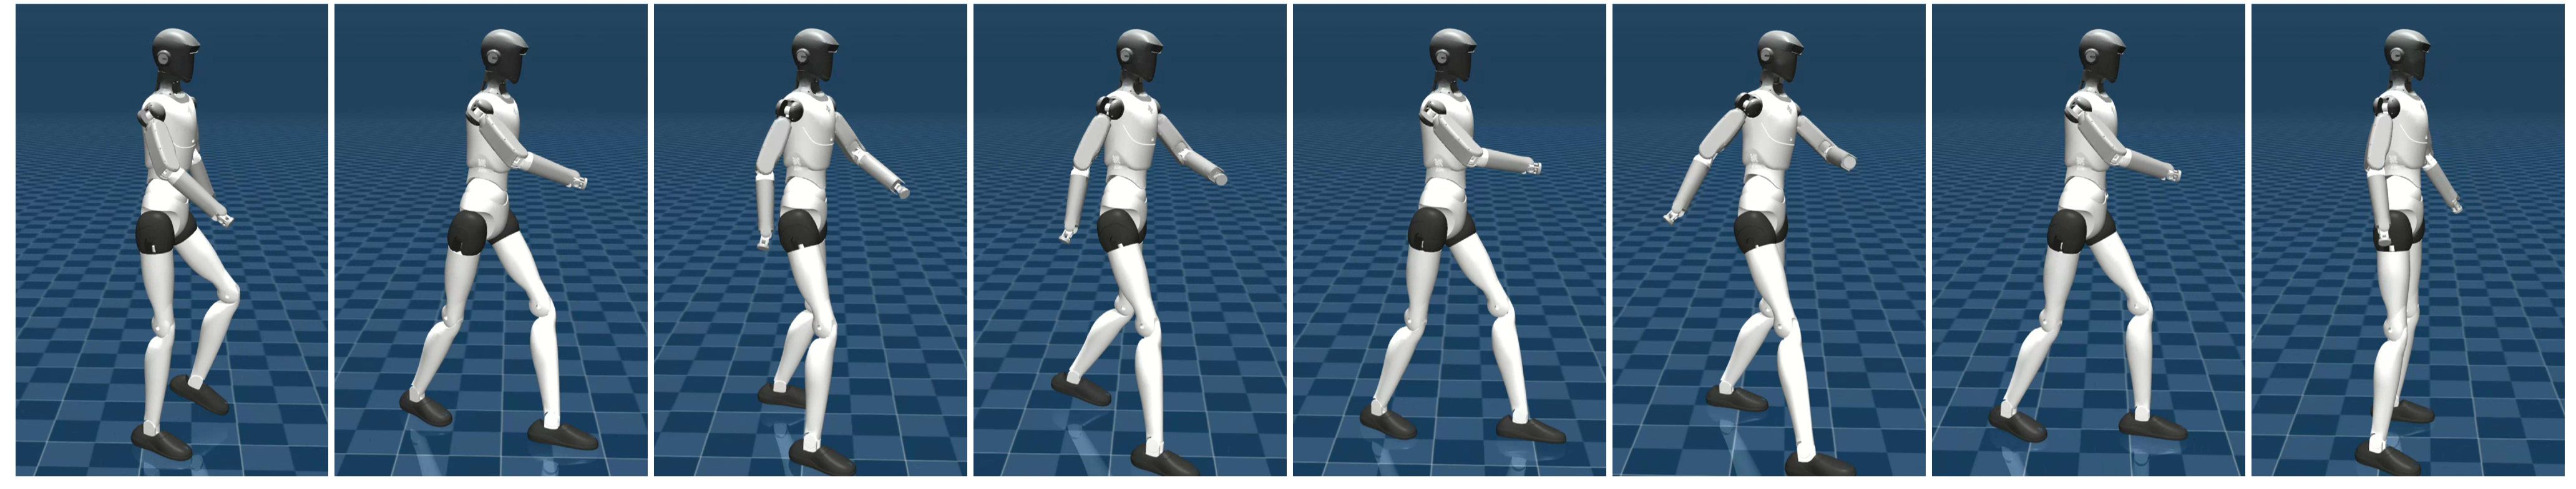
\includegraphics[width=\linewidth]{Figure/chapter4/walk_imitaion.png}
		\caption{行走动作跟踪}
	\end{subfigure}
	
	\vspace{0.5em}
	
	\begin{subfigure}{0.8\linewidth}
		\centering
		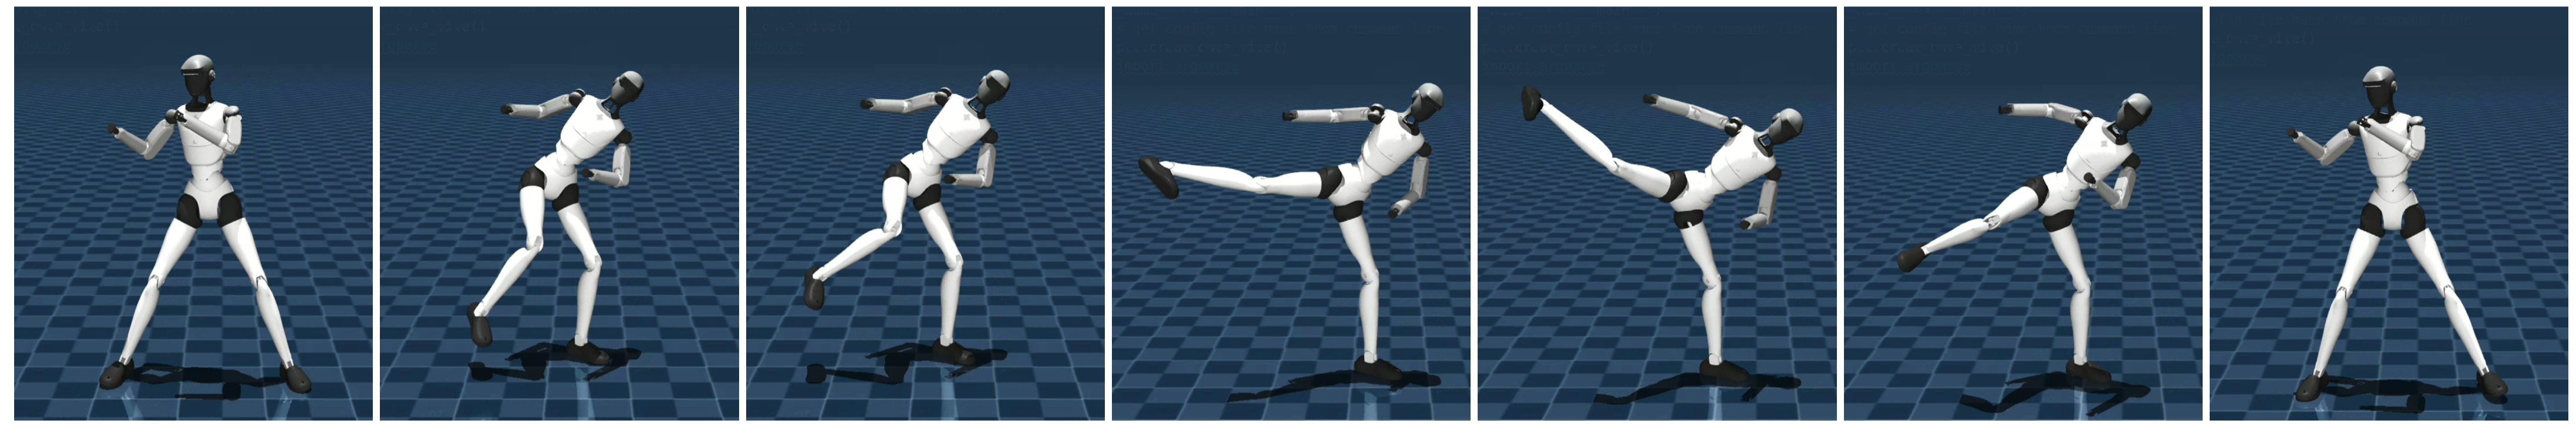
\includegraphics[width=\linewidth]{Figure/chapter4/kick_imitaion.png}
		\caption{侧踢动作跟踪}
	\end{subfigure}
	
	\vspace{0.5em}
	
	\begin{subfigure}{0.8\linewidth}
		\centering
		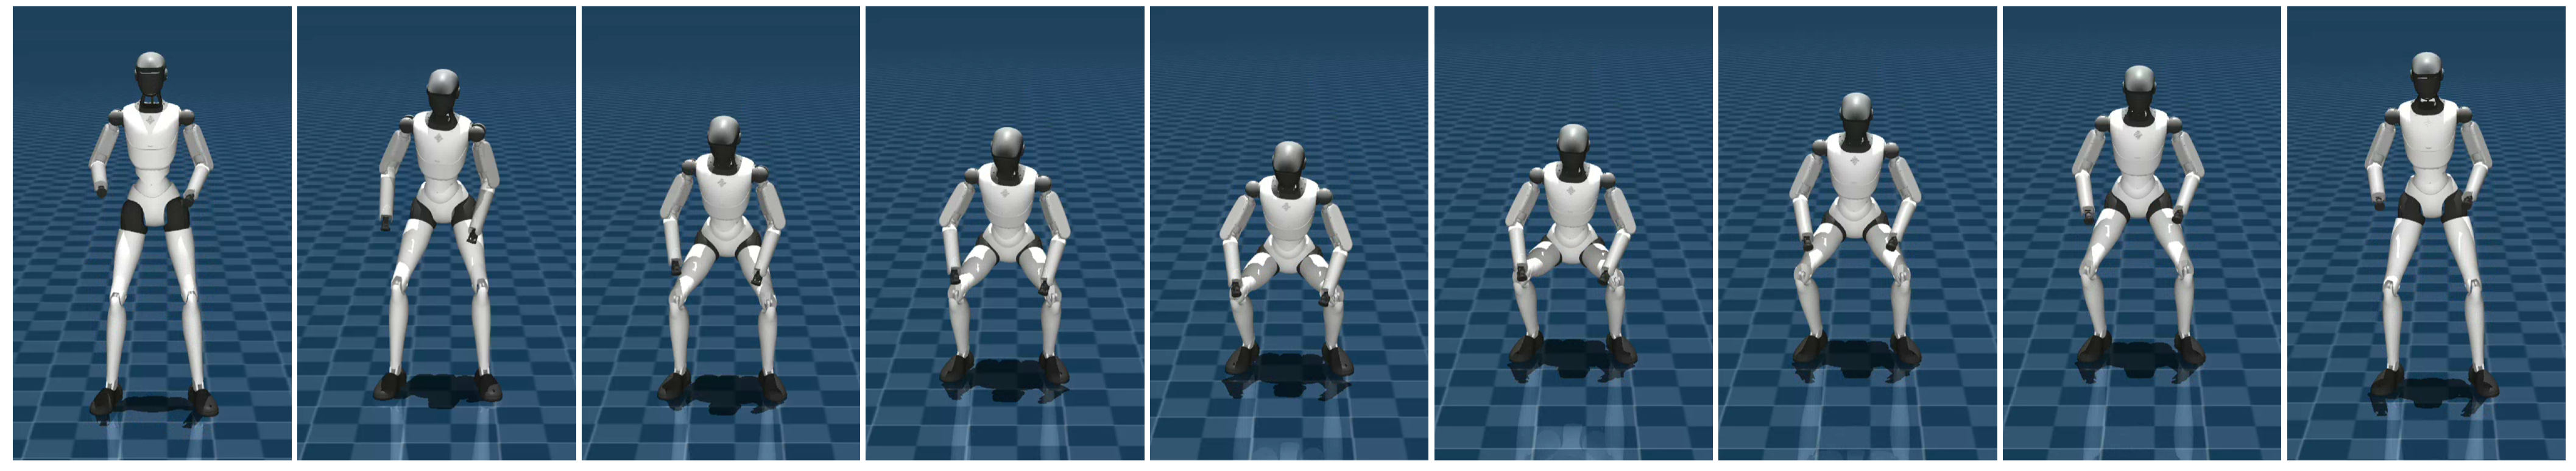
\includegraphics[width=\linewidth]{Figure/chapter4/pick_up.png}
		\caption{物体搬运动作跟踪}
	\end{subfigure}
	
	\vspace{0.8em}
	\caption{通用全身动作跟踪策略对参考动作的跟踪结果}
	\label{fig:imitation_results}
	
\end{figure}

在获得整体定性结果的基础上，进一步选取典型步态运动，对机器人下肢主要关节的轨迹跟踪效果进行定量分析。图~\ref{fig:gait_tracking} 给出了步态运动过程中左腿主要关节的角度变化曲线，其中蓝色实线表示机器人在仿真环境中的实际关节角，红色虚线表示对应的参考关节角。

可以观察到，在大部分时间段内，各关节的实际轨迹能够较好地跟随参考轨迹变化趋势，在相位、幅值以及周期性方面均保持较高一致性。这表明通用动作跟踪策略能够稳定地跟踪参考动作，并在动力学约束下复现参考运动模式。右腿关节轨迹呈现出与左腿类似的跟踪特性，因此本文仅展示其中一侧的结果。

具体而言，在髋关节俯仰与膝关节等主要驱动关节上，实际关节角与参考轨迹之间的误差较小，且峰值位置基本保持一致，说明策略能够较好地捕捉步态运动的关键动力学特征。对于踝关节，虽然在个别时刻存在一定幅度的偏差，但整体变化趋势仍与参考轨迹保持一致，这主要是由于足部与地面接触过程中接触动力学约束对关节运动产生的影响。

需要指出的是，在原始参考动作数据中，由于人体动作重定向误差以及动力学不一致等因素，部分关节轨迹可能存在抖动或局部不连续现象。为此，本文通过基于物理仿真的模仿学习过程对参考动作进行物理一致性修正，使得修正后的动作在满足机器人动力学约束的同时保持原始运动模式。实验结果表明，经物理修正后的运动轨迹在平滑性与稳定性方面均得到明显改善，从而为后续运动嵌入学习与高层策略训练提供了更加可靠的运动数据基础。

总体而言，底层通用全身动作跟踪策略能够在复杂动作条件下实现稳定且高精度的参考跟踪，并有效缓解原始数据中的噪声与不一致问题，为后续潜空间建模与高层策略学习提供可靠的动作执行基础。

\begin{figure}[htbp]
	\centering
	
	\begin{subfigure}{0.65\linewidth}
		\centering
		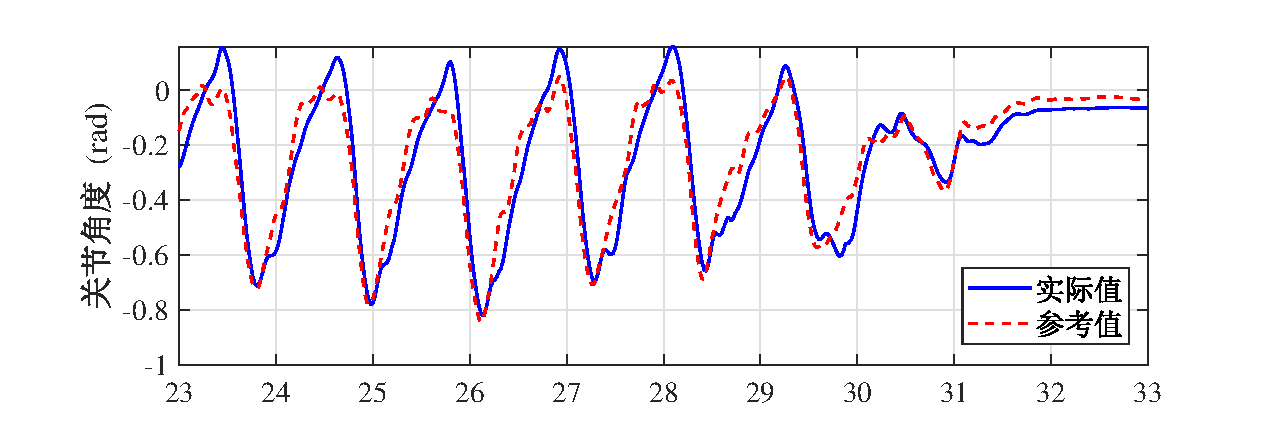
\includegraphics[width=\linewidth]{Figure/chapter4/track/hip_pitch.eps}
		\caption{}
	\end{subfigure}
	
	\vspace{0.3em}
	
	\begin{subfigure}{0.65\linewidth}
		\centering
		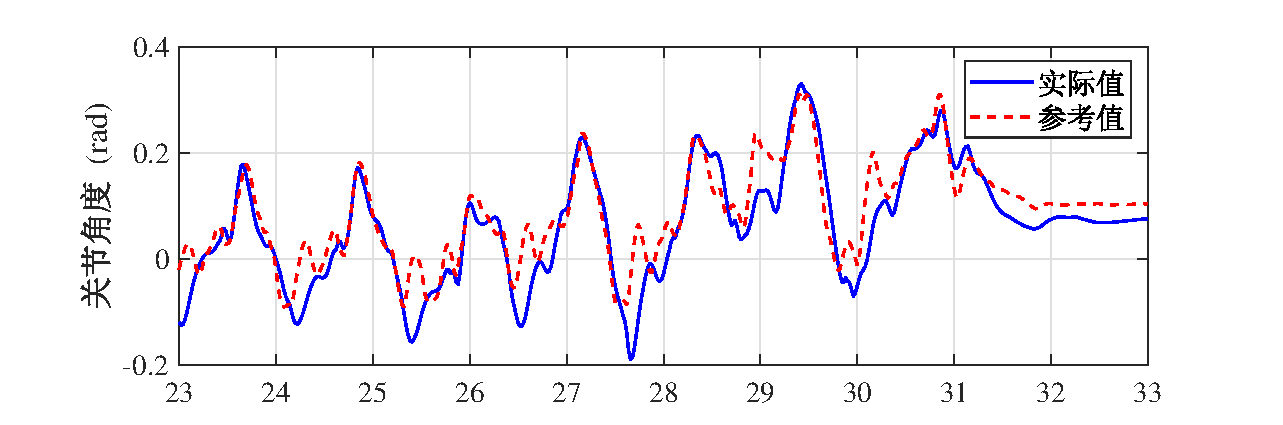
\includegraphics[width=\linewidth]{Figure/chapter4/track/hip_roll.eps}
		\caption{}
	\end{subfigure}
	
	\vspace{0.3em}
	
	\begin{subfigure}{0.65\linewidth}
		\centering
		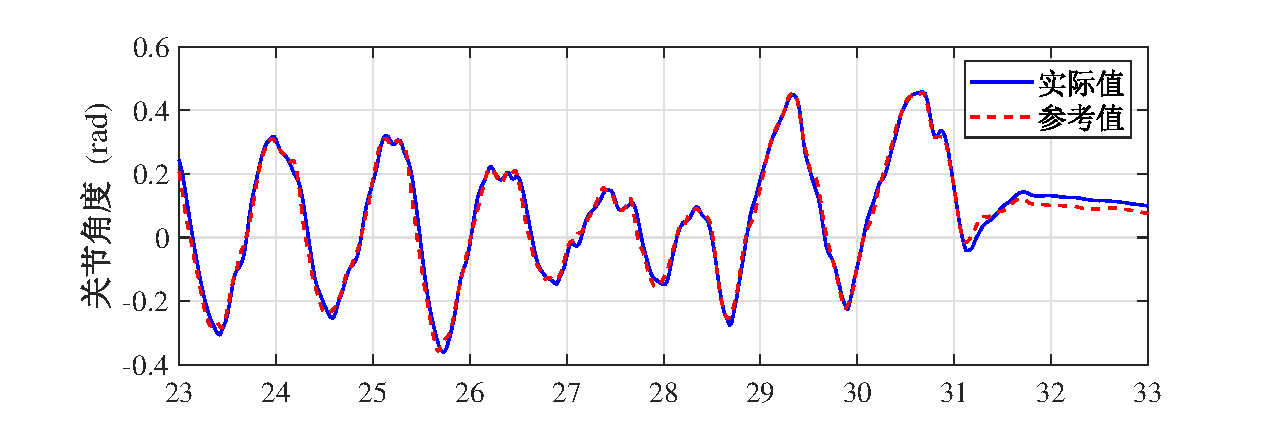
\includegraphics[width=\linewidth]{Figure/chapter4/track/hip_yaw.eps}
		\caption{}
	\end{subfigure}
	
	\vspace{0.3em}

	
	\begin{subfigure}{0.65\linewidth}
		\centering
		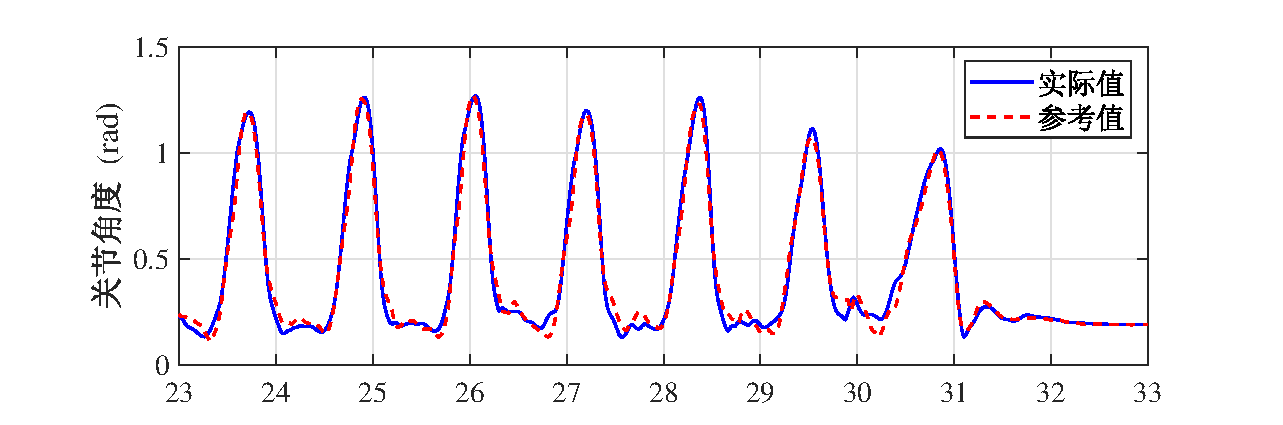
\includegraphics[width=\linewidth]{Figure/chapter4/track/knee.eps}
		\caption{}
	\end{subfigure}
	
	\vspace{0.3em}
	
	\begin{subfigure}{0.65\linewidth}
		\centering
		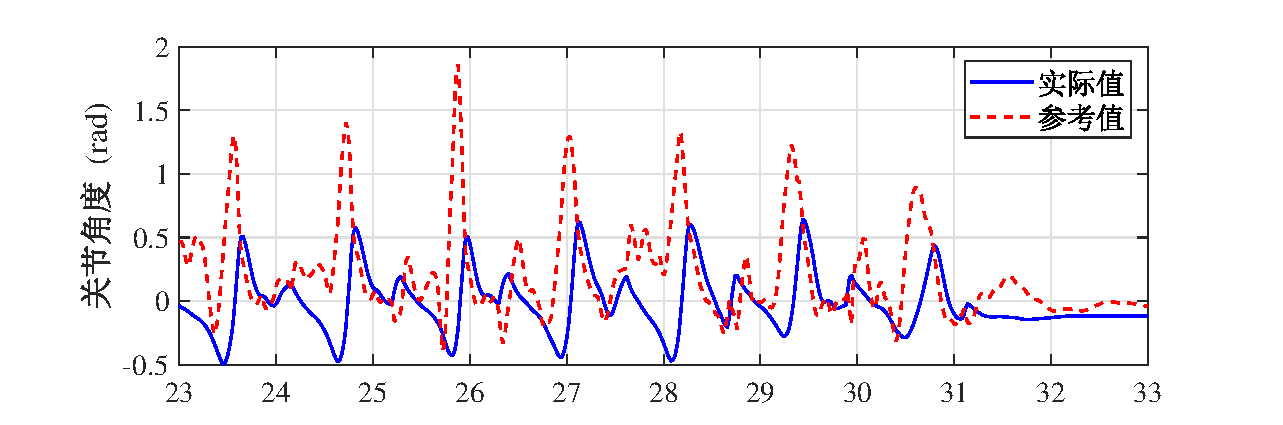
\includegraphics[width=\linewidth]{Figure/chapter4/track/ankle_pitch.eps}
		\caption{}
	\end{subfigure}
	
	\vspace{0.3em}
	
	\begin{subfigure}{0.65\linewidth}
		\centering
		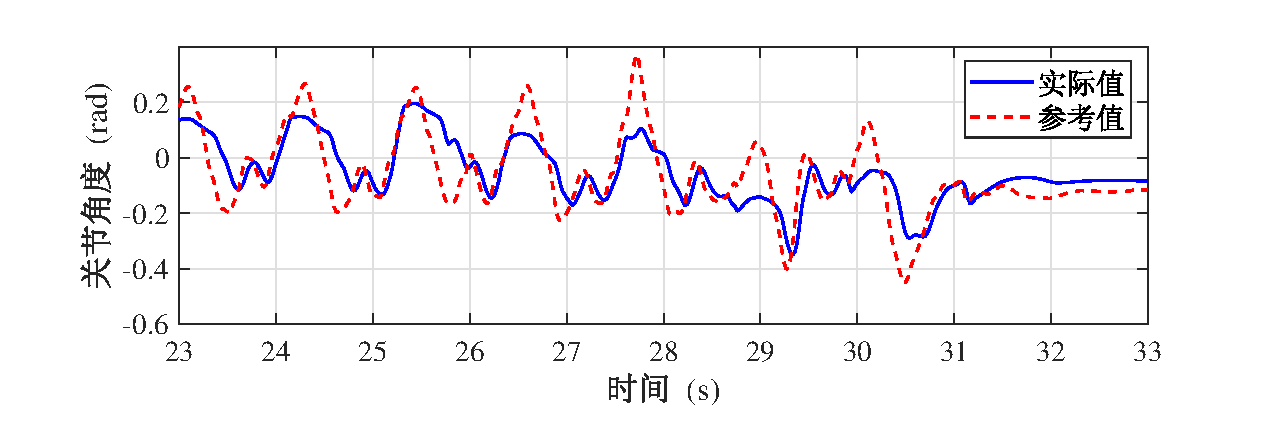
\includegraphics[width=\linewidth]{Figure/chapter4/track/ankle_roll.eps}
		\caption{}
	\end{subfigure}
	
	\vspace{0.4em}
	\caption{
		步态运动中下肢主要关节的轨迹跟踪结果。
		（a）髋关节前后摆；
		（b）髋关节侧摆；
		（c）髋关节旋转；
		（d）膝关节；
		（e）踝关节俯仰；
		（f）踝关节侧摆
	}
	\label{fig:gait_tracking}
	
\end{figure}


\subsection{基于MVAE的技能嵌入验证}

在获得稳定的底层动作跟踪能力之后，进一步验证所提出的基于 MVAE 的技能嵌入方法在动作表示与生成方面的有效性。具体而言，本节主要从动作表示质量、生成能力以及对下游控制性能的影响三个方面进行分析。

首先，将含有噪声的参考动作 $M_{\text{ref}}$ 进行物理一致性校正。通过低层通用动作跟踪策略在物理仿真环境中对参考轨迹进行模仿执行，从而消除原始动作中的动力学不一致与高频噪声，得到动力学一致的动作序列 $M_{\text{corr}}$。在此基础上，进一步利用 MVAE 对 $M_{\text{corr}}$ 进行建模，将其嵌入到一个连续且平滑的潜在动作空间中，得到动作表示 $M_{\text{vae}}$。该过程形成了从原始动作到物理一致动作再到潜空间表示的逐步优化链条。

在所学习的潜空间中，动作被建模为连续的状态转移序列，而未对动作片段进行显式划分或人工定义技能结构。尽管缺乏显式的技能划分约束，模型仍能够在潜空间中自动形成具有结构化特征的动作表示。当对解码器输入随机潜变量 $z$ 时，系统能够生成大量自然且连贯的全身运动。实验结果表明，生成动作在整体运动模式上与原始动作保持一致，同时在局部姿态细节上呈现一定变化，说明该潜在空间能够有效捕捉动作数据中的内在运动结构，并具备良好的泛化能力。

为了对不同阶段的运动数据质量进行定量评估，表~\ref{tab:motion_quality} 给出了参考动作 $M_{\text{ref}}$、物理修正后的动作 $M_{\text{corr}}$ 以及 MVAE 生成动作 $M_{\text{vae}}$ 的对比结果。可以观察到，经物理修正后的运动在动作平滑度与足部滑动指标上均得到显著改善，而经过 MVAE 嵌入后的动作在平滑性方面进一步提升。这表明，物理一致性修正与潜空间建模在去除动作噪声方面具有互补作用。

需要指出的是，MVAE 的平滑过程在一定程度上会引入额外的足部滑动现象，但该问题在后续通过低层策略在物理仿真环境中的模仿执行过程中得到有效缓解，从而保证最终生成动作的物理可行性与稳定性。

为了进一步分析物理修正机制对技能嵌入学习的影响，本文设计了对比实验：直接使用原始参考动作 $M_{\text{ref}}$ 训练 MVAE，并基于该潜空间训练高层策略（记为 w/o PhysicsCorr）。从表~\ref{tab:motion_quality} 可以看出，未进行物理修正的数据在动作平滑度与足部滑动方面表现较差。同时，表~\ref{tab:task_performance} 的结果表明，在缺乏物理一致性修正的情况下，高层策略在任务执行中的性能明显下降，尤其在末端执行器位置误差指标上退化更为显著。

上述结果表明，在构建高质量动作潜空间的过程中，引入基于物理的运动修正不仅能够提升潜在表示的平滑性与结构性，还对后续任务驱动的控制性能具有关键作用，是实现稳定分层控制的重要前提。

\begin{table}[htbp]
	\centering
	\caption{不同运动处理阶段的运动质量指标对比}
	\label{tab:motion_quality}
	\begin{tabular}{lccc}
		\toprule
		方法 & 动作平滑度（$10^3$ m/s$^3$） & 足部滑动（cm） & 跟踪误差（rad） \\
		\midrule
		$M_{\text{ref}}$ & 6.08 & 7.41 & 0.32 \\
		$M_{\text{corr}}$ & 3.14 & 1.46 & 0.18 \\
		$M_{\text{vae}}$ & 0.96 & 4.70 & 0.21 \\
		\midrule
		w/o PhysicsCorr & 1.19 & 2.82 & 0.24 \\
		Fed-full & \textbf{0.51} & \textbf{1.46} & \textbf{0.16} \\
		\bottomrule
	\end{tabular}
\end{table}

\subsection{分层全身控制方法验证}

在完成底层通用动作跟踪能力验证以及技能嵌入有效性验证之后，本节进一步从任务执行层面对所提出的分层全身控制框架进行验证。该验证的核心目标在于考察：高层策略是否能够在 MVAE 潜空间中生成合理的潜变量，并通过低层跟踪控制器将其转化为能够服务于具体任务目标的连续全身动作。

为全面评估所提出系统框架在运动生成与任务执行中的性能，本文设计了三个具有代表性的控制任务，包括目标位置移动、末端目标到达以及物体搬运。这些任务分别对应全身导航、精细末端控制以及腿臂协同操作三类典型场景，能够从不同角度评估机器人在复杂任务中对多种运动技能的调用、组合与规划能力。

\paragraph{目标位置移动任务}

该任务要求机器人从初始位置移动至指定目标位置 $x^*$。为了提高策略的泛化能力，目标位置在机器人周围一定范围内随机采样。该任务的奖励函数定义为：
\begin{equation}
	r_t^G=\exp\left(-0.5\|x_t^{\text{root}}-x^*\|^2\right),
\end{equation}
其中，$x_t^{\text{root}}$ 表示机器人在 $t$ 时刻根节点在世界坐标系中的位置，$x^*$ 表示目标位置。

\paragraph{末端目标到达任务}

目标到达任务用于评估机器人在精细运动控制方面的能力。在该任务中，机器人需要控制末端执行器移动到指定目标位置 $x^*$。目标位置在机器人可达工作空间内随机生成。该任务的奖励函数定义为：
\begin{equation}
	r_t^G=\exp\left(-2\|x_t^{\text{ee}}-x^*\|^2\right),
\end{equation}
其中，$x_t^{\text{ee}}$ 表示机器人末端执行器在 $t$ 时刻在世界坐标系中的位置。

\paragraph{物体搬运任务}

物体搬运任务用于评估机器人在腿臂协同控制场景中的能力。在该任务中，机器人需要移动至目标物体附近并完成抓取。该任务要求机器人在接近目标物体的过程中协调下肢运动与上肢操作，从而验证所提出控制框架在全身协同控制场景中的有效性。该任务的奖励函数定义为：
\begin{equation}
	r_t^G=\exp\left(-2.5\|x_t^{\text{hand}}-x_t^{\text{obj}}\|^2\right),
\end{equation}
其中，$x_t^{\text{hand}}$ 表示机器人末端执行器在 $t$ 时刻在世界坐标系中的位置，$x_t^{\text{obj}}$ 表示目标物体在 $t$ 时刻在世界坐标系中的位置，$\alpha_o$ 为奖励尺度系数。

在完整分层控制框架下，高层策略在 MVAE 潜空间中生成潜变量，并通过解码器产生目标姿态序列，而低层模仿控制策略负责在物理仿真环境中跟踪这些参考动作。图~\ref{fig:task_results} 展示了分层控制框架在不同任务中的执行结果。可以观察到，机器人能够在目标位置移动、目标到达以及物体搬运等不同任务场景下完成相应控制目标，且部分由 MVAE 生成的动作示例在任务执行过程中得到了体现。

从整体执行效果来看，高层策略能够根据任务需求在潜空间中生成具有行为差异的潜变量，并通过解码器产生具有连续性的目标动作序列；与此同时，低层控制器能够对这些目标动作进行稳定跟踪，从而使机器人完成复杂任务。该结果表明，所提出的分层控制框架能够实现从潜空间技能表示到物理动作执行的有效衔接，并支持不同基础运动技能在任务过程中的组合与复用。

\begin{figure}[htbp]
	\centering
	
	\subfloat[目标位置移动任务]{
		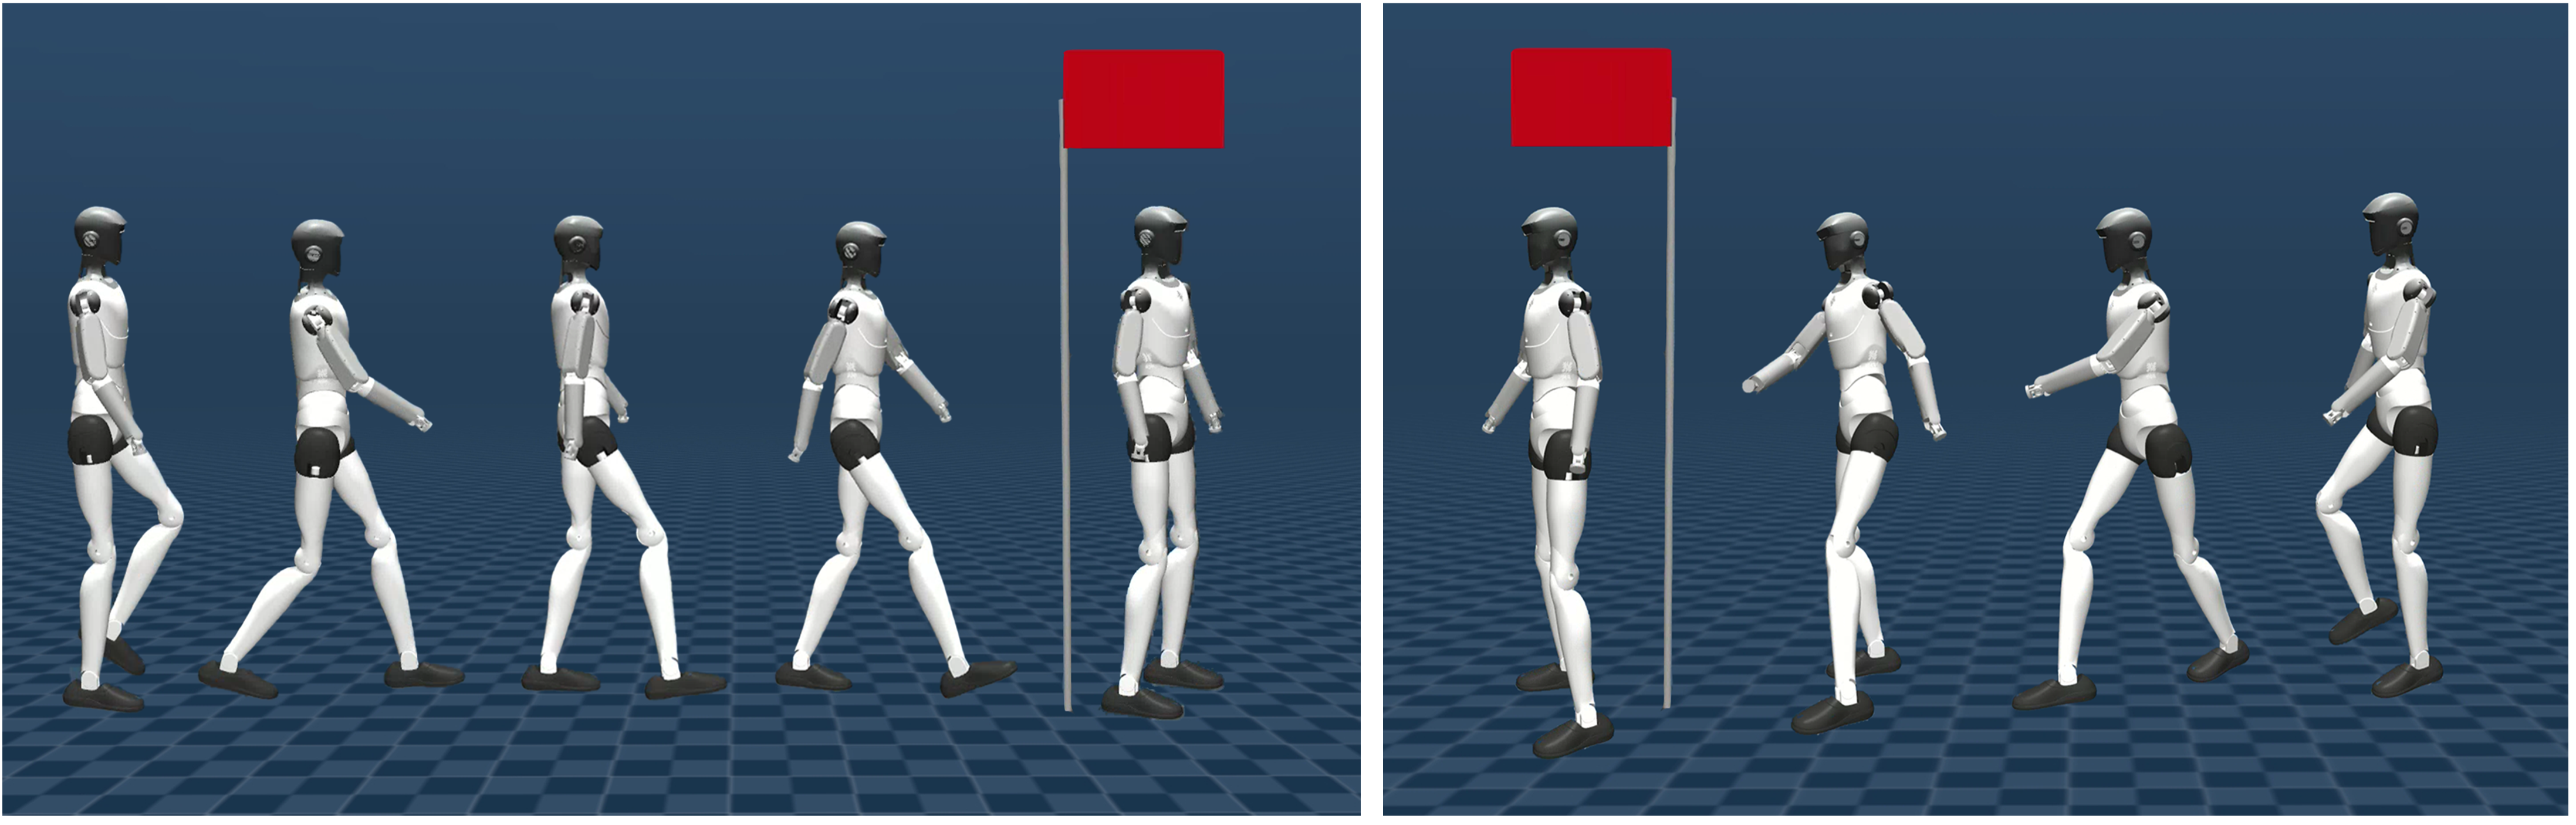
\includegraphics[width=0.9\linewidth]{Figure/chapter4/walk_loco.png}}
	
	\vspace{0.5em}
	
	\subfloat[目标到达任务]{
		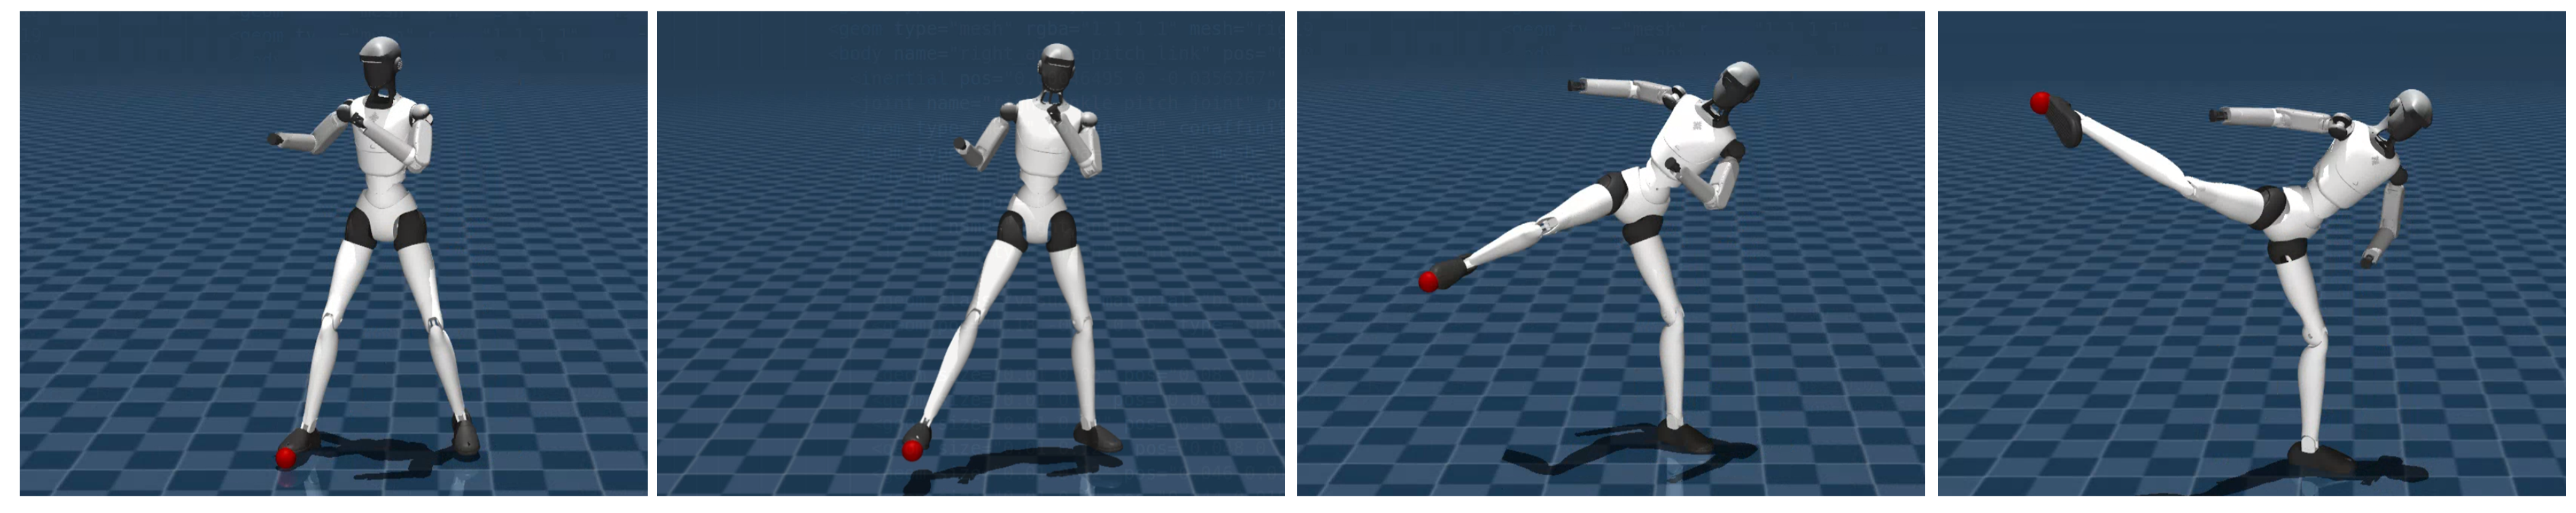
\includegraphics[width=0.9\linewidth]{Figure/chapter4/kick_box.png}}
	
	\vspace{0.5em}
	
	\subfloat[物体搬运任务]{
		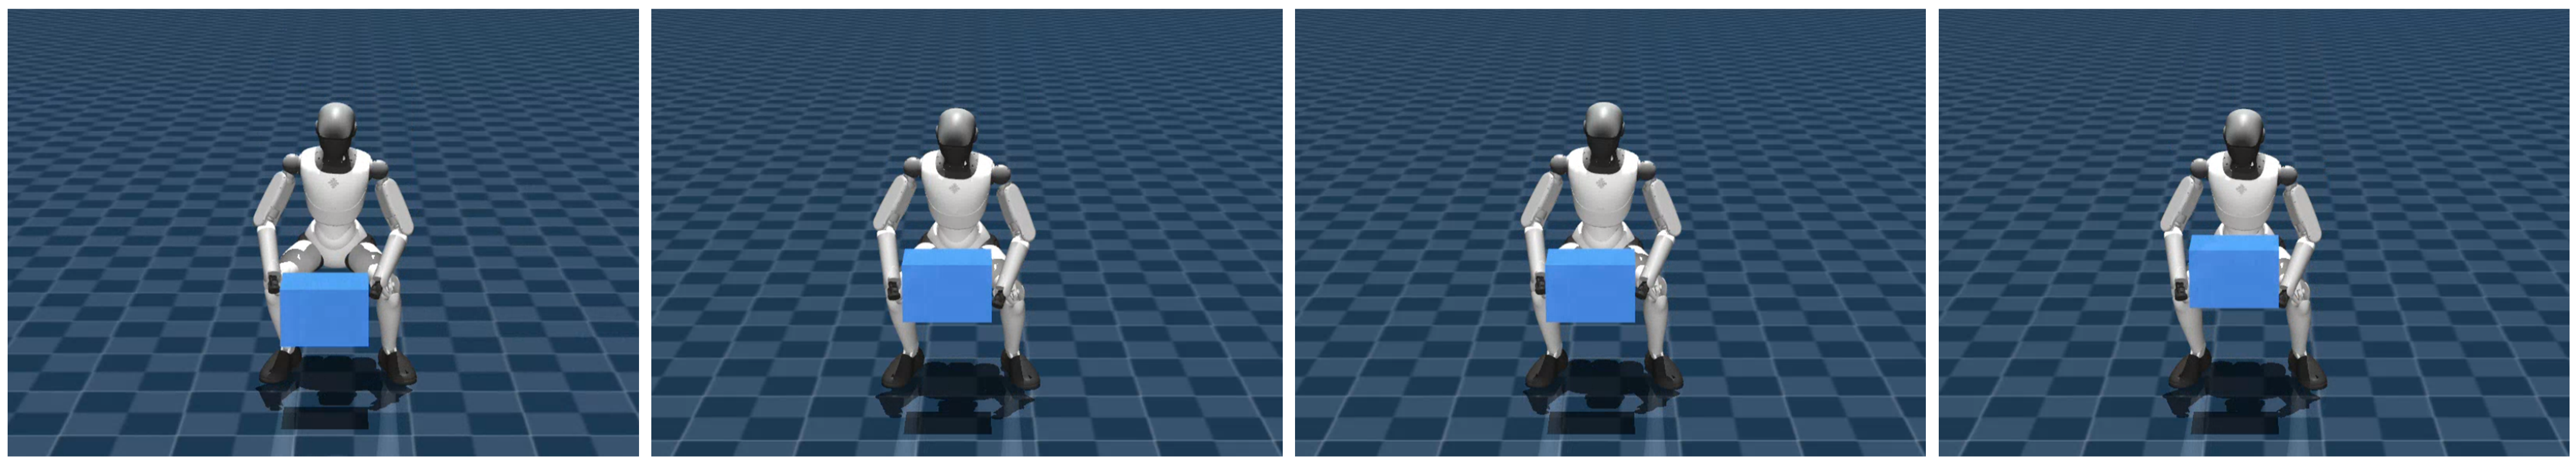
\includegraphics[width=0.9\linewidth]{Figure/chapter4/pickup_box.png}}
	
	\vspace{0.8em}
	\caption{分层控制框架在不同任务中的执行结果。}
	\label{fig:task_results}
	
\end{figure}

为了进一步评估所提出控制框架在目标位置移动任务中的表现，图~\ref{fig:loco_traj} 给出了机器人在多个目标位置条件下的运动轨迹示意图。其中，红色圆点表示任务中随机生成的目标位置，黑色圆点表示机器人最终到达的位置，灰色虚线表示机器人在执行任务过程中的运动轨迹。

从任务完成结果来看，在大多数测试场景中，机器人能够沿着连续且平滑的路径逐步接近目标位置，并最终停留在目标区域附近。虽然在个别目标点处机器人最终位置与目标位置之间存在一定偏差，但整体误差保持在较小范围内，表明所学习到的控制策略能够有效完成目标位置移动任务。

进一步分析运动轨迹可以发现，机器人在不同目标位置之间移动时能够保持良好的运动连贯性与稳定性，未出现明显的轨迹振荡或路径不连续现象。这表明所学习的控制策略在不同空间目标之间能够实现平滑过渡，并具备稳定的运动规划与执行能力。

\begin{figure}[htbp]
	\centering
	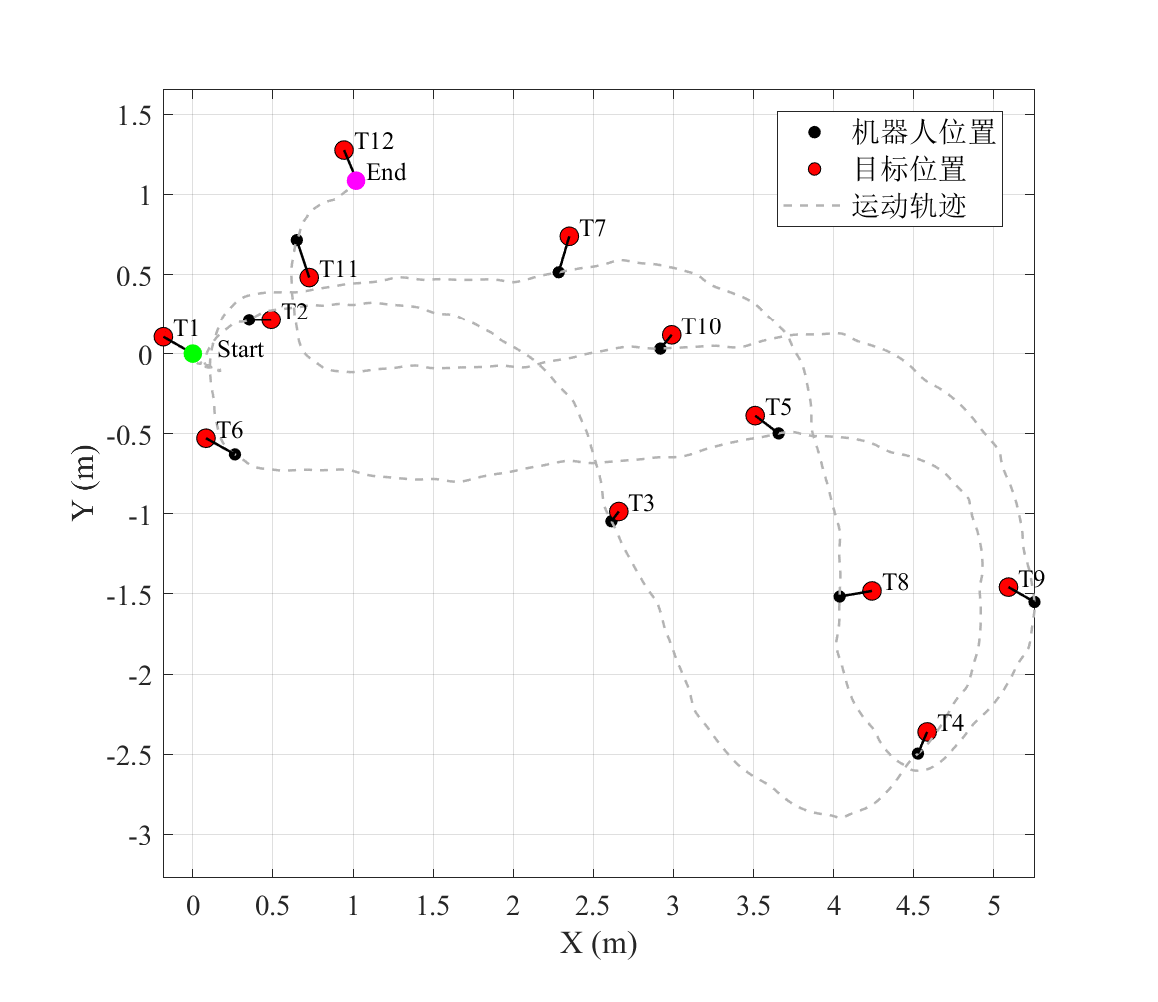
\includegraphics[width=0.8\linewidth]{Figure/chapter4/loco_pos.eps}
	\caption{目标位置移动任务中的机器人运动轨迹示意图。}
	\label{fig:loco_traj}
\end{figure}

从定量指标上看，机器人在该任务中的成功率较高，同时目标位置误差保持在较小范围内（见表~\ref{tab:task_performance}），进一步验证了所提出控制方法在导航类全身运动任务中的有效性。

为了进一步评估所提出控制框架在物体搬运任务中的执行效果，图~\ref{fig:carry_traj} 给出了机器人在完成物体搬运过程时左右手末端执行器的三维运动轨迹。其中，蓝色曲线表示左手末端轨迹，橙色曲线表示右手末端轨迹，黄色曲线表示在接触到物体后末端执行器的运动路径。

\begin{figure}[htbp]
	\centering
	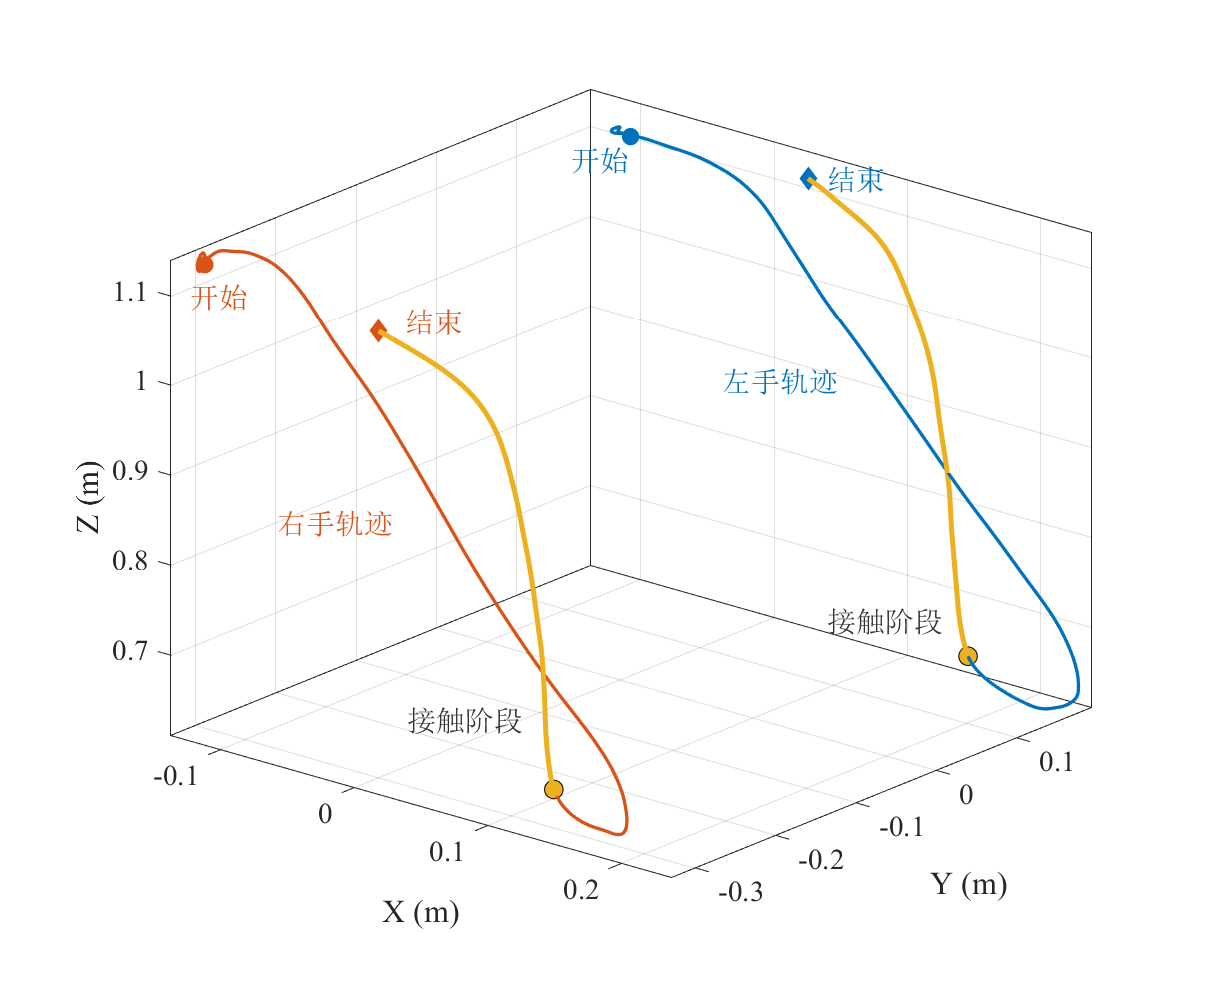
\includegraphics[width=0.85\linewidth]{Figure/chapter4/pick_up_tra.eps}
	\caption{物体搬运任务中双手末端执行器的三维运动轨迹。}
	\label{fig:carry_traj}
\end{figure}

可以观察到，在任务开始阶段，机器人双臂末端从初始位置出发，并沿着平滑连续的轨迹逐渐接近目标物体。当末端执行器与物体接触后，轨迹进入接触阶段，此时双手轨迹呈现出较为稳定的协同运动模式，从而实现对物体的搬运。随后，机器人继续沿规划轨迹将物体移动至目标位置。

从整体轨迹变化可以看出，左右手末端轨迹在空间中保持较好的协调关系，且轨迹变化连续平滑，没有出现明显的振荡或突变现象。这表明所提出的控制框架能够在保持全身运动稳定性的同时，实现双臂末端的协同控制，从而完成复杂的物体搬运任务。

此外，在接触阶段中，末端轨迹变化相对缓慢且稳定，说明策略在物体接触过程中能够保持较好的控制精度与稳定性，从而避免由于接触动力学不稳定而导致的任务失败。该结果进一步验证了所提出分层控制框架在双臂协同操作任务中的有效性。

从定量指标上看，该任务在测试场景中取得了较高的任务成功率，并保持较小的目标位置误差（见表~\ref{tab:task_performance}），进一步验证了所提出方法在复杂操作任务中的鲁棒性与有效性。

最后，为进一步分析分层全身控制框架中关键模块对任务性能的影响，本文开展了消融实验，结果如表~\ref{tab:task_performance} 所示。对比完整方法（Fed-full）与去除物理修正（w/o PhysicsCorr）以及去除混合控制机制（w/o HybridCtr）两种简化方法可以发现，完整框架在目标位置移动成功率、目标到达误差以及物体搬运成功率等指标上均取得了最优结果。

其中，去除物理修正后，动作潜空间的输入数据质量下降，导致高层规划生成的动作在物理一致性与任务执行精度方面均受到影响；而去除混合控制机制后，系统在高层任务驱动与低层动作执行之间的衔接能力减弱，从而导致整体任务性能下降。上述结果说明，物理一致性修正与混合控制机制对于提升分层控制框架的任务执行能力均具有重要作用。

\begin{table}[htbp]
	\centering
	\caption{消融实验：物理修正（PhysicsCorr）与混合控制（HybridCtr）对任务性能的影响}
	\label{tab:task_performance}
	\begin{tabular}{lccc}
		\toprule
		方法 & 位置移动成功率 & 目标到达误差 (cm) & 物体搬运成功率 \\
		\midrule
		w/o PhysicsCorr & 0.81 & 6.32 & 0.74 \\
		w/o HybridCtr & 0.73 & 8.45 & 0.66 \\
		Fed-full & \textbf{0.90} & \textbf{4.18} & \textbf{0.83} \\
		\bottomrule
	\end{tabular}
\end{table}

综上所述，所提出的分层全身控制框架能够在不同任务场景中实现运动技能的有效调用、组合与调度，并在任务执行过程中保持良好的稳定性、自然性与鲁棒性。实验结果表明，该方法能够实现从潜空间技能表示到高层任务规划再到底层动作执行的完整闭环，为类人机器人在复杂场景中的腿臂协同控制提供了有效支撑。




\section{本章小结}

本章在第三章通用全身动作跟踪控制策略的基础上，针对类人机器人在复杂任务场景中需要执行多种运动行为并实现灵活切换的问题，提出了一种基于技能嵌入的分层全身控制方法。

在方法设计方面，首先在底层构建通用全身动作跟踪控制器。通过对不同类别动作训练专家策略，并结合数据聚合（DAgger）进行策略蒸馏，获得统一的通用跟踪策略，使机器人能够在物理约束下稳定复现多样化参考动作。其次，在中间表示层引入基于自回归条件变分自编码器（MVAE）的运动生成模型，对参考动作进行建模，在低维潜空间中构建连续且紧凑的运动技能表示。进一步地，在高层规划层中，通过在潜空间中进行策略学习，并结合关节空间残差修正机制，实现了从任务目标到动作生成再到底层执行的分层控制结构，从而支持多种运动技能的组合与平滑过渡。

在系统鲁棒性方面，针对机器人在实际运行过程中可能出现的跌倒问题，设计了基于强化学习的恢复策略。通过对多种随机初始姿态进行训练，使机器人能够从任意跌倒姿态恢复至稳定站立状态，并在恢复后重新进入任务执行流程，从而增强系统在复杂环境下的连续运行能力。

在仿真验证中，围绕目标位置移动、末端目标到达及物体搬运等任务，对所提出方法进行了系统评估。实验结果表明：在任务性能方面，所提出方法在各类任务中均取得较高成功率（如目标位置移动任务成功率达到 90\%），并保持较低的目标误差（如末端到达误差约为 4.18\,cm）；在运动质量方面，生成动作具有良好的平滑性与稳定性，关节跟踪误差与足部滑动均控制在较低水平。同时，消融实验结果表明，物理一致性修正与混合控制机制对提升任务执行精度与成功率具有关键作用。

综上所述，本章提出的基于技能嵌入的分层全身控制方法能够在统一框架下实现运动技能的有效表示、组合与调度，并在复杂任务场景中保持良好的控制性能与系统鲁棒性，为类人机器人在多任务环境中的腿臂协同控制提供了一种可行且有效的技术路径。


